%!TEX root = ../template.tex
%%%%%%%%%%%%%%%%%%%%%%%%%%%%%%%%%%%%%%%%%%%%%%%%%%%%%%%%%%%%%%%%%%%%
%% chapter3.tex
%% NOVA thesis document file
%%
%% Chapter with a short latex tutorial and examples
%%%%%%%%%%%%%%%%%%%%%%%%%%%%%%%%%%%%%%%%%%%%%%%%%%%%%%%%%%%%%%%%%%%%

\typeout{NT FILE chapter3.tex}%

\makeatletter
\newcommand{\ntifpkgloaded}{%
  \@ifpackageloaded%
}
\makeatother


\chapter{Experiment}
\label{cha:experiment}

\epigraph{
	"Somewhere, something incredible is waiting to be known."
}{Carl Sagan}



\section{Context and Goal of the Experiment} % (fold)
\label{sec:contex_goal_experiment}

The proposed experiment, detailed in research proposal G-24-00249, aims to investigate the structure of the neutron-rich fluorine isotope, $^{25}$F, through one-proton knockout reactions. This study is motivated by the "drastic extension of the neutron drip line for Z=9 compared to Z=8 isotopes," a phenomenon that remains poorly understood \cite{ahn_location_2019}. The experiment seeks to elucidate how the $^{24}$O core is polarized by the presence of an additional proton in $^{25}$F, thereby shedding light on the mechanisms responsible for the observed drip line extension.

The experiment will employ the quasi-free scattering (QFS) reaction $^{25}$F(p,2p)$^{24}$O in inverse kinematics, effectively knocking out a deeply bound valence proton from the $^{25}$F nucleus \cite{panin_exclusive_2016}. This approach will utilize the R3B experimental setup, including the high-efficiency neutron detector NeuLAND, to achieve complete kinematic measurements and obtain accurate spectroscopic information on the populated final states of $^{24}$O \cite{boretzky_neuland_2021}. By analyzing the experimental data, researchers aim to determine the extent to which the single d5/2 proton in $^{25}$F modifies the structure of the core nucleons, potentially indicating deformation or polarization of the $^{24}$O core \cite{macchiavelli_core_2020}.

Ultimately, the goal of this experiment is to provide a more detailed understanding of the nuclear structure of neutron-rich fluorine isotopes and the underlying reasons for the extended neutron drip line at Z=9. The results will contribute to a more comprehensive picture of nuclear forces and structure in exotic nuclei, addressing a fundamental question in nuclear physics.


\section{The GSI Accelerator System}

\gls{GSI}

\gls{GSI}

\gls{FRS}

\gls{FRS}

\subsection{Beam}

Primary Beam: 40Ar 700 MeV/u

Beryllium Target at FRS -> Creates cocktail beam with 25F

Liquid Hidrogen Target in Cave C in center of CALIFA

\section{R3B Setup}

\gls{R3B}

\gls{R3B}

\gls{ToFD}

\gls{ToFD}

\gls{NeuLAND}

\gls{NeuLAND}

\gls{GLAD}

\gls{GLAD}

\gls{CALIFA}

\gls{CALIFA}

\gls{RPC}

\gls{RPC}
\begin{figure}
	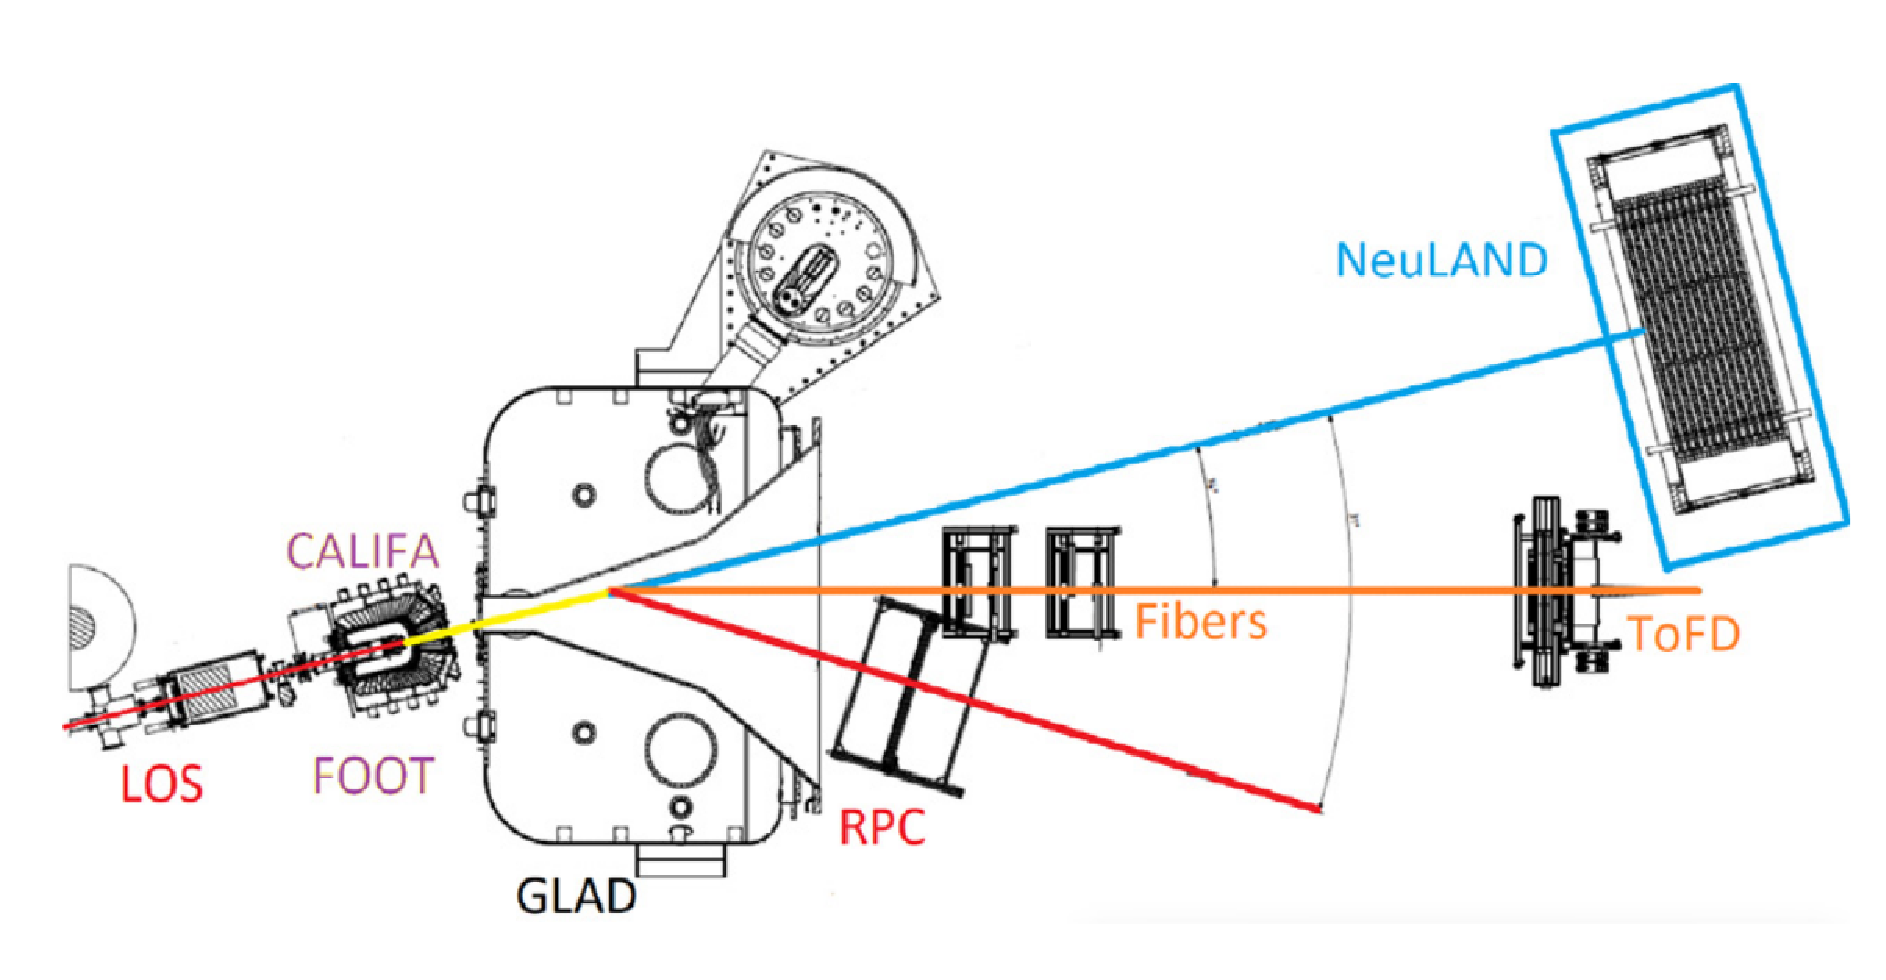
\includegraphics[width=\linewidth]{SchematicR3BSetup}
	\caption{Schematic representation of the R3B setup.}
	\label{fig:R3BSetup}
\end{figure}



\subsection{Role of each detector}

\subsubsection{MWPCs}

\subsubsection{TwinMUSIC}

\subsubsection{LOS (Large-area Optical System)}

Function: Measures the time of flight (ToF) and beam position.

How it works:

\begin{itemize}
	\item Uses fast scintillators and photomultipliers (PMTs).
	\item Provides a reference start signal for ToF measurements.
	\item Crucial for precise velocity determination of incoming beam particles.
\end{itemize}

Importance: Helps in identifying incoming beam particles before they interact with the target.


\subsubsection{ROLU}

\subsubsection{CALIFA (CALorimeter for In-Flight detection of γ-rays and light charged particles)}

Function: A gamma-ray and charged-particle calorimeter surrounding the reaction target.

Structure:

\begin{itemize}
	\item High granularity for precise energy and angle measurements.
	\item Covers nearly 4π around the reaction point.
\end{itemize}


Detects:

\begin{itemize}
	\item γ-rays from nuclear de-excitation.
	\item Light charged particles (e.g., protons, alphas).
	\item Helps in reconstructing excited states of nuclear fragments.
\end{itemize}

- Technology:

\begin{itemize}
	\item CsI(Tl) scintillators coupled to SiPMs or PMTs.
	\item High energy resolution for γ-ray spectroscopy.
\end{itemize}


\subsubsection{FOOTs}

\subsubsection{GLAD (GSI Large Acceptance Dipole Magnet)}

Function: Bends charged particles to determine their momentum.

Key properties:

\begin{itemize}
	\item Superconducting dipole magnet.
	\item Large acceptance ($\sim$80 msr) to handle high-energy reaction products.
	\item Used in combination with tracking detectors to reconstruct fragment momenta.
\end{itemize}

Why it’s important:

\begin{itemize}
	\item Essential for measuring momentum distributions, a key observable in QFS and knockout reactions.
	\item Helps reconstruct the missing momentum of removed nucleons.
\end{itemize}


\subsubsection{NeuLAND (New Large-Area Neutron Detector)}

Function: Detects neutrons produced in nuclear reactions \cite{boretzky_neuland_2021}.

Why it's crucial:

\begin{itemize}
	\item Neutron knockout and quasi-free scattering involve neutron-rich final states.
	\item Neutron detection is challenging but necessary for reconstructing the full reaction kinematics.
\end{itemize}


Technology:

\begin{itemize}
	\item Plastic scintillator bars with time-of-flight (ToF) measurement.
	\item Very fast response ($\sim$100 ps time resolution) to distinguish multiple neutrons.
	\item Large area ($\sim$30 m$^2$) to maximize detection efficiency.
\end{itemize}

What it measures:

\begin{itemize}
	\item Neutron energy via ToF.
	\item Angular distribution of emitted neutrons.
\end{itemize}

Advantage:

\begin{itemize}
	\item Much improved over its predecessor LAND \cite{blaich_large_1992}, providing higher detection efficiency for multi-neutron events.
\end{itemize}


\subsubsection{Fiber Trackers}

Function: Track charged particles after the reaction.

Technology:

\begin{itemize}
	\item Consists of plastic scintillating fibers.
	\item Read out by SiPMs (Silicon Photomultipliers).
\end{itemize}

Why it matters:

\begin{itemize}
	\item Provides precise position information.
	\item Works in conjunction with other tracking detectors to reconstruct fragment trajectories.
\end{itemize}


\subsubsection{ToFD (Time-of-Flight Detector)}

Function: Measures the velocity of charged fragments for mass identification \cite{heil_new_2022}.

Why it’s needed:

\begin{itemize}
	\item In QFS and fragmentation reactions, products have different masses and need to be distinguished.
	\item ToF combined with tracking and momentum measurement allows isotope separation.
\end{itemize}

Technology:

\begin{itemize}
	\item Plastic scintillators with fast timing resolution ($\sim$50 ps).
	\item High-speed photomultiplier tubes (PMTs) for precise ToF measurements.
\end{itemize}



\subsection{Particular Role of RPC}

\cite{xarepe_resistive_2023}


\subsection{Main DAQ}

Each detector is connected to the main \gls{DAQ}, everytime they have a trigger, they send a trigger request to the main \gls{DAQ}. If multiple detectors send a trigger request, it is considered an event to register and the main \gls{DAQ} sends an accept signal, allowing every detector to save that signal.

All of these saved signals of each detector are then saved in a common \textit{lmd} file containing every detectors data separated by event.

There's a synchronization signal with around 10 Hz to make sure every detector is synchronized.


\section{Personal Contribution to the Experiment}